\begin{frame}[fragile]{Now Let's Build a Core!}

  \begin{enumerate}
    \item<1-> Make all pincell universes
    \begin{itemize}
      \item<1-> Fuel rod, control rod, burnable absorber, etc.
    \end{itemize}
    \item<2-> Make assembly pin-lattices
    \begin{itemize}
      \item<2-> Different enrichment assemblies, different burnable absorber configurations, etc.
    \end{itemize}
    \item<3-> Make core assembly-lattice
  \end{enumerate}

  \centering
  \onslide<3->{See input xml files in examples/demos/plotting}
  
  \vspace{0.2cm}
  
  \centering
  \begin{tikzpicture}
    \onslide<1->\draw[fill=blue!70!white] (-1,-1) rectangle (1,1);
    \onslide<1->\draw[fill=gray] (0,0) circle (0.7258);
    \onslide<1->\draw[fill=yellow] (0,0) circle (0.63508);
    \onslide<1->\draw[fill=red] (0,0) circle (0.62250);

    \onslide<2->\draw[thick,->] (1.2,0) -- (2.0,0);
    \begin{scope}[shift={(5.3,0)}, transform canvas={scale=0.7}]
      \begin{scope}[shift={(-1,-1)}]
        \onslide<2->\draw[fill=blue!70!white] (-1,-1) rectangle (1,1);
        \onslide<2->\draw[fill=gray] (0,0) circle (0.7258);
        \onslide<2->\draw[fill=yellow] (0,0) circle (0.63508);
        \onslide<2->\draw[fill=green] (0,0) circle (0.62250);
      \end{scope}
      \begin{scope}[shift={(1,-1)}]
        \onslide<2->\draw[fill=blue!70!white] (-1,-1) rectangle (1,1);
        \onslide<2->\draw[fill=gray] (0,0) circle (0.7258);
        \onslide<2->\draw[fill=yellow] (0,0) circle (0.63508);
        \onslide<2->\draw[fill=red] (0,0) circle (0.62250);
      \end{scope}
      \begin{scope}[shift={(-1,1)}]
        \onslide<2->\draw[fill=blue!70!white] (-1,-1) rectangle (1,1);
        \onslide<2->\draw[fill=gray] (0,0) circle (0.7258);
        \onslide<2->\draw[fill=yellow] (0,0) circle (0.63508);
        \onslide<2->\draw[fill=red] (0,0) circle (0.62250);
      \end{scope}
      \begin{scope}[shift={(1,1)}]
        \onslide<2->\draw[fill=blue!70!white] (-1,-1) rectangle (1,1);
        \onslide<2->\draw[fill=gray] (0,0) circle (0.7258);
        \onslide<2->\draw[fill=yellow] (0,0) circle (0.63508);
        \onslide<2->\draw[fill=green] (0,0) circle (0.62250);
      \end{scope}
    \end{scope}
    
    \onslide<3->\draw[thick,->] (5.3,0) -- (6.1,0);
    \onslide<3->\node[anchor=west] at (6.2,0){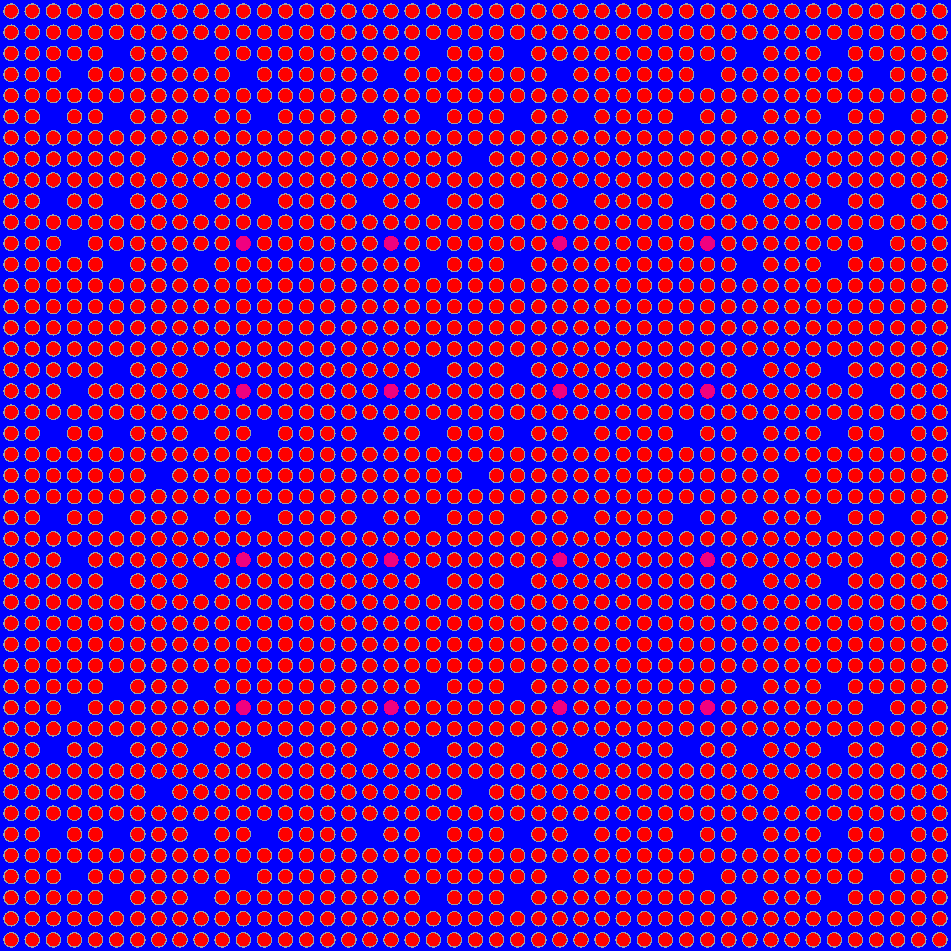
\includegraphics[width=1.5in]{src/smallcore.png}};
  \end{tikzpicture}

\end{frame}

%-------------------------------------------------------------------------------

\begin{frame}[fragile]{Pincells}

  \begin{scriptsize}
    \begin{lstlisting}[language=XML,gobble=4]
      
      <!-- Blank Water Universe -->
      <surface id="99" type="sphere"     coeffs="0.0 0.0 0.0 400.0"/>   <!-- dummy -->
      <cell id="11" universe="1" material="1" surfaces="-99"/>
      <cell id="12" universe="1" material="1" surfaces=" 99"/>

      <!-- Fuel Rod -->
      <surface id="1"  type="z-cylinder" coeffs="0.0 0.0 0.514858"/>    <!-- fuel OR      -->
      <surface id="2"  type="z-cylinder" coeffs="0.0 0.0 0.602996"/>    <!-- fuel clad OR -->
      <cell id="21" universe="2" material="2" surfaces="  -1"/>         <!-- fuel  -->
      <cell id="22" universe="2" material="3" surfaces="1 -2"/>         <!-- clad  -->
      <cell id="23" universe="2" material="1" surfaces="   2"/>         <!-- water -->

      <!-- Control Rod -->
      <surface id="3"  type="z-cylinder" coeffs="0.0 0.0 0.585000"/>    <!-- pyrex OR -->
      <cell id="31" universe="3" material="4" surfaces="  -3"/>         <!-- pyrex -->
      <cell id="32" universe="3" material="1" surfaces="   3"/>         <!-- water -->
      
    \end{lstlisting}
  \end{scriptsize}

    
\end{frame}

%-------------------------------------------------------------------------------

\begin{frame}[fragile]{Pin-Lattices}

  \centering

  Central Fuel Assembly

  \begin{scriptsize}
    \begin{lstlisting}[language=XML,gobble=4]
      <!-- Central Fuel Assembly -->      
      <lattice id="11" type="rectangular" dimension="15 15">
        <lower_left> -12.2682 -12.2682 </lower_left>
        <width>    1.63576 1.63576 </width>
        <universes>
          2 2 2 2 2 2 2 2 2 2 2 2 2 2 2
          2 2 2 2 2 2 2 2 2 2 2 2 2 2 2
          2 2 2 2 2 1 2 2 2 1 2 2 2 2 2
          2 2 2 3 2 2 2 2 2 2 2 3 2 2 2
          2 2 2 2 2 2 2 2 2 2 2 2 2 2 2
          2 2 1 2 2 1 2 2 2 1 2 2 1 2 2
          2 2 2 2 2 2 2 2 2 2 2 2 2 2 2
          2 2 2 2 2 2 2 1 2 2 2 2 2 2 2
          2 2 2 2 2 2 2 2 2 2 2 2 2 2 2
          2 2 1 2 2 1 2 2 2 1 2 2 1 2 2
          2 2 2 2 2 2 2 2 2 2 2 2 2 2 2
          2 2 2 3 2 2 2 2 2 2 2 3 2 2 2
          2 2 2 2 2 1 2 2 2 1 2 2 2 2 2
          2 2 2 2 2 2 2 2 2 2 2 2 2 2 2
          2 2 2 2 2 2 2 2 2 2 2 2 2 2 2
        </universes>
      </lattice>
      <cell id="111" universe="111" fill="11" surfaces=""/>
    \end{lstlisting}
  \end{scriptsize}
  
\end{frame}

%-------------------------------------------------------------------------------

\begin{frame}[fragile]{Pin-Lattices}

  \centering

  North, South, East, and West Assemblies

  \begin{scriptsize}
    \begin{lstlisting}[language=XML,gobble=4]
      <!-- North Fuel Assembly -->      
      <lattice id="22" type="rectangular" dimension="15 15">
        <lower_left> -12.2682 -12.2682 </lower_left>
        <width>    1.63576 1.63576 </width>
        <universes>
          2 2 2 2 2 2 2 2 2 2 2 2 2 2 2
          2 2 2 2 2 2 2 2 2 2 2 2 2 2 2
          2 2 2 2 2 1 2 2 2 1 2 2 2 2 2
          2 2 2 1 2 2 2 2 2 2 2 1 2 2 2
          2 2 2 2 2 2 2 2 2 2 2 2 2 2 2
          2 2 1 2 2 1 2 2 2 1 2 2 1 2 2
          2 2 2 2 2 2 2 2 2 2 2 2 2 2 2
          2 2 2 2 2 2 2 1 2 2 2 2 2 2 2
          2 2 2 2 2 2 2 2 2 2 2 2 2 2 2
          2 2 1 2 2 1 2 2 2 1 2 2 1 2 2
          2 2 2 2 2 2 2 2 2 2 2 2 2 2 2
          2 2 2 3 2 2 2 2 2 2 2 3 2 2 2
          2 2 2 2 2 1 2 2 2 1 2 2 2 2 2
          2 2 2 2 2 2 2 2 2 2 2 2 2 2 2
          2 2 2 2 2 2 2 2 2 2 2 2 2 2 2
        </universes>
      </lattice>
      <cell id="222" universe="222" fill="22" surfaces=""/>                     <!-- north -->
      <cell id="444" universe="444" fill="222" surfaces="" rotation="0 0 90"/>  <!-- west  -->
      <cell id="555" universe="555" fill="222" surfaces="" rotation="0 0 180"/> <!-- south -->
      <cell id="666" universe="666" fill="222" surfaces="" rotation="0 0 270"/> <!-- east  -->
    \end{lstlisting}
  \end{scriptsize}
  
\end{frame}

%-------------------------------------------------------------------------------

\begin{frame}[fragile]{Pin-Lattices}

  \centering

  Northeast, Southeast, Northwest, and Southwest Assemblies

  \begin{scriptsize}
    \begin{lstlisting}[language=XML,gobble=4]
      <!-- Northeast Fuel Assembly -->      
      <lattice id="33" type="rectangular" dimension="15 15">
        <lower_left> -12.2682 -12.2682 </lower_left>
        <width>    1.63576 1.63576 </width>
        <universes>
          2 2 2 2 2 2 2 2 2 2 2 2 2 2 2
          2 2 2 2 2 2 2 2 2 2 2 2 2 2 2
          2 2 2 2 2 1 2 2 2 1 2 2 2 2 2
          2 2 2 1 2 2 2 2 2 2 2 1 2 2 2
          2 2 2 2 2 2 2 2 2 2 2 2 2 2 2
          2 2 1 2 2 1 2 2 2 1 2 2 1 2 2
          2 2 2 2 2 2 2 2 2 2 2 2 2 2 2
          2 2 2 2 2 2 2 1 2 2 2 2 2 2 2
          2 2 2 2 2 2 2 2 2 2 2 2 2 2 2
          2 2 1 2 2 1 2 2 2 1 2 2 1 2 2
          2 2 2 2 2 2 2 2 2 2 2 2 2 2 2
          2 2 2 3 2 2 2 2 2 2 2 1 2 2 2
          2 2 2 2 2 1 2 2 2 1 2 2 2 2 2
          2 2 2 2 2 2 2 2 2 2 2 2 2 2 2
          2 2 2 2 2 2 2 2 2 2 2 2 2 2 2
        </universes>
      </lattice>
      <cell id="333" universe="333" fill="33" surfaces=""/>                     <!-- NE -->
      <cell id="777" universe="777" fill="333" surfaces="" rotation="0 0 90"/>  <!-- NW -->
      <cell id="888" universe="888" fill="333" surfaces="" rotation="0 0 180"/> <!-- SE -->
      <cell id="999" universe="999" fill="333" surfaces="" rotation="0 0 270"/> <!-- SW -->
    \end{lstlisting}
  \end{scriptsize}
  
\end{frame}

%-------------------------------------------------------------------------------

\begin{frame}[fragile]{Core-Lattice and Main Universe}

  \centering

  Done!

  \begin{scriptsize}
    \begin{lstlisting}[language=XML,gobble=4]
    <!-- Core lattice -->
    <lattice id="99" type="rectangular" dimension="3 3">
      <lower_left> -36.8046 -36.8046 </lower_left>
      <width>   24.5364  24.5364 </width>
      <universes>
        777 222 333
        444 111 666
        888 555 999
      </universes>
    </lattice>
    
    <!-- Main Universe -->
    <surface id="10" type="x-plane" coeffs="-36.8046" boundary="vacuum"/>
    <surface id="20" type="x-plane" coeffs=" 36.8046" boundary="vacuum"/>
    <surface id="30" type="y-plane" coeffs="-36.8046" boundary="vacuum"/>
    <surface id="40" type="y-plane" coeffs=" 36.8046" boundary="vacuum"/>
    <surface id="50" type="z-plane" coeffs="-80.0000" boundary="vacuum"/>
    <surface id="60" type="z-plane" coeffs=" 80.0000" boundary="vacuum"/>
    
    <cell id="1000" universe="0" fill="99" surfaces="10 -20 30 -40 50 -60"/>
    
    \end{lstlisting}
  \end{scriptsize}
  
\end{frame}

